%% notes-tex/027-metabolic-flux-module/sections/5-measured.tex
%% [[experiments.026-metabolism-flux.enzyme-constrained-thermodynamic-flux-layer]]
%% https://github.com/Mjvolk3/torchcell/tree/main/notes-tex/027-metabolic-flux-module/sections/5-measured.tex

\section{What has been measured\secstatus{todo}}
\label{sec:measured}

\subsection{What separates the two rounds\secstatus{todo}}

Both rounds ask whether the flux module helps predict betaxanthin, and they differ in
almost everything else. Reading a number from one against a number from the other is the
mistake this table exists to prevent.

\begin{table}[H]
  \centering
  \footnotesize
  \caption[026 against 027]{The two rounds, side by side. The backbone is the difference
  that outranks the others, since the 026 baseline was roughly five times below the
  demonstrated ceiling on this target.}
  \label{tab:026v027}
  %% SOURCE: experiments/026-metabolism-flux/scripts/sweep_flux.py and its results/sweep_*.json
  %% args block; experiments/027-betaxanthin-metabolic/conf/base.yaml and scripts/train_bx.py.
  \begin{tabular}{@{}p{0.20\textwidth}p{0.36\textwidth}p{0.36\textwidth}@{}}
    \hline
    & 026 & 027 \\
    \hline
    backbone & weak: 2 graphs, learnable embeddings, hidden 32, 4 heads &
      strong: 9 graphs, \texttt{prot\_T5\_all}, no learnable table, hidden 90, 9 heads \\
    trainer & \texttt{sweep\_flux.py} & \texttt{train\_bx.py} \\
    epochs & 30 & 200 \\
    split & re-rolled per seed, so seed moves signal and nuisance together &
      \textbf{pinned} Merzbacher 639-gene test split, fixed across every cell \\
    scored on & validation, \textbf{maximum over epochs} &
      test, at an epoch selected on validation \\
    replication & 10 seeds per arm, plus a 24-run permuted-label null &
      24 seeds per arm, with the nulls as two of the six arms \\
    machine & GilaHyper & Delta \texttt{gpuA40x4}, 72 workers \\
    W\&B project & \texttt{torchcell\_026\_flux\_sweep} & \texttt{torchcell\_027\_bxfx} \\
    outcome & no arm clears its own null & every cell is a constant predictor \\
    \hline
  \end{tabular}
\end{table}

\subsection{The 026 sweep, and why it decided nothing\secstatus{todo}}

\begin{table}[H]
  \centering
  \footnotesize
  \caption[026 arm results]{The 026 sweep on betaxanthin. The statistic is validation
  Pearson scored as a \emph{maximum over epochs}, which is an upward-biased order
  statistic, and the last column is the mean of the final five epochs, which is not.}
  \label{tab:026}
  %% SOURCE: experiments/026-metabolism-flux/results/flux_arms_summary.json
  \begin{tabular}{@{}lrrrrr@{}}
    \hline
    Arm & Seeds & Peak mean & s.e.m. & Peak epoch & Last-5 mean \\
    \hline
    \texttt{flux\_anchored} & 10 & 0.1151 & 0.0095 & 17 & 0.0057 \\
    \texttt{flux\_free} & 10 & 0.1020 & 0.0115 & 12 & 0.0212 \\
    \texttt{flux\_off} & 10 & 0.0837 & 0.0112 & 10 & 0.0044 \\
    \texttt{pooled} & 10 & 0.0416 & 0.0098 & 4 & $-0.0041$ \\
    \texttt{flux\_nullspace} & 10 & 0.0381 & 0.0114 & 0 & 0.0000 \\
    \hline
  \end{tabular}
\end{table}

Every run behind that table has a W\&B page, indexed in Table~\ref{tab:wandb-runs-026};
the arm rows there are the ten seeds each arm contributes, and the null and regularization
grids are the runs the next two paragraphs draw on.

%% GENERATED by experiments/026-metabolism-flux/scripts/wandb_run_index.py
%% from results/sweep_*.json. Do not edit by hand; rerun the script.
%% SOURCE: experiments/026-metabolism-flux/results/sweep_arms_a.json, sweep_arms_b.json,
%% sweep_null.json, sweep_reg_flux_anchored.json (wandb_run_id, wandb_url per run).
\begin{table}[H]
  \centering
  \footnotesize
  \caption[W\&B runs of the 026 sweep]{Every run of the 026 sweep behind Table~\ref{tab:026}, 98 in all, in project \href{https://wandb.ai/zhao-group/torchcell_026_flux_sweep}{\texttt{torchcell\_026\_flux\_sweep}} (entity \texttt{zhao-group}). One row per grid cell; each entry is a seed and its run id, linked to the run page. The 18 earlier runs in \texttt{flux\_arms\_gpu*.json} predate W\&B logging and have no page.}
  \label{tab:wandb-runs-026}
  \begin{tabular}{@{}llp{0.60\textwidth}@{}}
    \hline
    Grid & Cell & Seed: run \\
    \hline
    \texttt{arms} & \texttt{flux\_anchored} & 101: \href{https://wandb.ai/zhao-group/torchcell_026_flux_sweep/runs/u3iq97id}{\texttt{u3iq97id}} 102: \href{https://wandb.ai/zhao-group/torchcell_026_flux_sweep/runs/ot19w48c}{\texttt{ot19w48c}} 103: \href{https://wandb.ai/zhao-group/torchcell_026_flux_sweep/runs/g3iazwin}{\texttt{g3iazwin}} 104: \href{https://wandb.ai/zhao-group/torchcell_026_flux_sweep/runs/4mx9l38a}{\texttt{4mx9l38a}} 105: \href{https://wandb.ai/zhao-group/torchcell_026_flux_sweep/runs/gzs9e901}{\texttt{gzs9e901}} 106: \href{https://wandb.ai/zhao-group/torchcell_026_flux_sweep/runs/1gav5w61}{\texttt{1gav5w61}} 107: \href{https://wandb.ai/zhao-group/torchcell_026_flux_sweep/runs/p8i6sp2v}{\texttt{p8i6sp2v}} 108: \href{https://wandb.ai/zhao-group/torchcell_026_flux_sweep/runs/qm9fddw2}{\texttt{qm9fddw2}} 109: \href{https://wandb.ai/zhao-group/torchcell_026_flux_sweep/runs/c4i363am}{\texttt{c4i363am}} 110: \href{https://wandb.ai/zhao-group/torchcell_026_flux_sweep/runs/kbc0h7bv}{\texttt{kbc0h7bv}} \\
     & \texttt{flux\_free} & 101: \href{https://wandb.ai/zhao-group/torchcell_026_flux_sweep/runs/oyppbowh}{\texttt{oyppbowh}} 102: \href{https://wandb.ai/zhao-group/torchcell_026_flux_sweep/runs/8h54lhih}{\texttt{8h54lhih}} 103: \href{https://wandb.ai/zhao-group/torchcell_026_flux_sweep/runs/hum6hv7i}{\texttt{hum6hv7i}} 104: \href{https://wandb.ai/zhao-group/torchcell_026_flux_sweep/runs/rdqxfngq}{\texttt{rdqxfngq}} 105: \href{https://wandb.ai/zhao-group/torchcell_026_flux_sweep/runs/gi56ouut}{\texttt{gi56ouut}} 106: \href{https://wandb.ai/zhao-group/torchcell_026_flux_sweep/runs/3j67e7ou}{\texttt{3j67e7ou}} 107: \href{https://wandb.ai/zhao-group/torchcell_026_flux_sweep/runs/3v3j67wv}{\texttt{3v3j67wv}} 108: \href{https://wandb.ai/zhao-group/torchcell_026_flux_sweep/runs/yepgwwki}{\texttt{yepgwwki}} 109: \href{https://wandb.ai/zhao-group/torchcell_026_flux_sweep/runs/5q0zos2c}{\texttt{5q0zos2c}} 110: \href{https://wandb.ai/zhao-group/torchcell_026_flux_sweep/runs/flkf5wzn}{\texttt{flkf5wzn}} \\
     & \texttt{flux\_nullspace} & 101: \href{https://wandb.ai/zhao-group/torchcell_026_flux_sweep/runs/lw7cdqt5}{\texttt{lw7cdqt5}} 102: \href{https://wandb.ai/zhao-group/torchcell_026_flux_sweep/runs/boqtw6j0}{\texttt{boqtw6j0}} 103: \href{https://wandb.ai/zhao-group/torchcell_026_flux_sweep/runs/wgv3ogwk}{\texttt{wgv3ogwk}} 104: \href{https://wandb.ai/zhao-group/torchcell_026_flux_sweep/runs/3x9sgbve}{\texttt{3x9sgbve}} 105: \href{https://wandb.ai/zhao-group/torchcell_026_flux_sweep/runs/87j1nvb4}{\texttt{87j1nvb4}} 106: \href{https://wandb.ai/zhao-group/torchcell_026_flux_sweep/runs/dgojsxba}{\texttt{dgojsxba}} 107: \href{https://wandb.ai/zhao-group/torchcell_026_flux_sweep/runs/fay4r3sn}{\texttt{fay4r3sn}} 108: \href{https://wandb.ai/zhao-group/torchcell_026_flux_sweep/runs/zw2up11b}{\texttt{zw2up11b}} 109: \href{https://wandb.ai/zhao-group/torchcell_026_flux_sweep/runs/e7cbxan6}{\texttt{e7cbxan6}} 110: \href{https://wandb.ai/zhao-group/torchcell_026_flux_sweep/runs/m1h0dbd2}{\texttt{m1h0dbd2}} \\
     & \texttt{flux\_off} & 101: \href{https://wandb.ai/zhao-group/torchcell_026_flux_sweep/runs/cvghzlru}{\texttt{cvghzlru}} 102: \href{https://wandb.ai/zhao-group/torchcell_026_flux_sweep/runs/875pwhhp}{\texttt{875pwhhp}} 103: \href{https://wandb.ai/zhao-group/torchcell_026_flux_sweep/runs/74ucn3q9}{\texttt{74ucn3q9}} 104: \href{https://wandb.ai/zhao-group/torchcell_026_flux_sweep/runs/d6fufo9v}{\texttt{d6fufo9v}} 105: \href{https://wandb.ai/zhao-group/torchcell_026_flux_sweep/runs/90m94xzu}{\texttt{90m94xzu}} 106: \href{https://wandb.ai/zhao-group/torchcell_026_flux_sweep/runs/qx017bn6}{\texttt{qx017bn6}} 107: \href{https://wandb.ai/zhao-group/torchcell_026_flux_sweep/runs/1epiwuli}{\texttt{1epiwuli}} 108: \href{https://wandb.ai/zhao-group/torchcell_026_flux_sweep/runs/0klqi5gj}{\texttt{0klqi5gj}} 109: \href{https://wandb.ai/zhao-group/torchcell_026_flux_sweep/runs/luid55f0}{\texttt{luid55f0}} 110: \href{https://wandb.ai/zhao-group/torchcell_026_flux_sweep/runs/29p85yl7}{\texttt{29p85yl7}} \\
     & \texttt{pooled} & 101: \href{https://wandb.ai/zhao-group/torchcell_026_flux_sweep/runs/czltmzp7}{\texttt{czltmzp7}} 102: \href{https://wandb.ai/zhao-group/torchcell_026_flux_sweep/runs/amie33pg}{\texttt{amie33pg}} 103: \href{https://wandb.ai/zhao-group/torchcell_026_flux_sweep/runs/7pxleywm}{\texttt{7pxleywm}} 104: \href{https://wandb.ai/zhao-group/torchcell_026_flux_sweep/runs/h9o1xexz}{\texttt{h9o1xexz}} 105: \href{https://wandb.ai/zhao-group/torchcell_026_flux_sweep/runs/71ftm5fd}{\texttt{71ftm5fd}} 106: \href{https://wandb.ai/zhao-group/torchcell_026_flux_sweep/runs/561svy7h}{\texttt{561svy7h}} 107: \href{https://wandb.ai/zhao-group/torchcell_026_flux_sweep/runs/pq8nj79f}{\texttt{pq8nj79f}} 108: \href{https://wandb.ai/zhao-group/torchcell_026_flux_sweep/runs/u4nh0znr}{\texttt{u4nh0znr}} 109: \href{https://wandb.ai/zhao-group/torchcell_026_flux_sweep/runs/bw06snzd}{\texttt{bw06snzd}} 110: \href{https://wandb.ai/zhao-group/torchcell_026_flux_sweep/runs/60ks7mhg}{\texttt{60ks7mhg}} \\
    \hline
    \texttt{null} & \texttt{flux\_anchored} & 301: \href{https://wandb.ai/zhao-group/torchcell_026_flux_sweep/runs/avo7djgs}{\texttt{avo7djgs}} 302: \href{https://wandb.ai/zhao-group/torchcell_026_flux_sweep/runs/adcfdc1w}{\texttt{adcfdc1w}} 303: \href{https://wandb.ai/zhao-group/torchcell_026_flux_sweep/runs/io7ugt8m}{\texttt{io7ugt8m}} 304: \href{https://wandb.ai/zhao-group/torchcell_026_flux_sweep/runs/xy8srp0b}{\texttt{xy8srp0b}} 305: \href{https://wandb.ai/zhao-group/torchcell_026_flux_sweep/runs/qv527rhn}{\texttt{qv527rhn}} 306: \href{https://wandb.ai/zhao-group/torchcell_026_flux_sweep/runs/up6z1xil}{\texttt{up6z1xil}} 307: \href{https://wandb.ai/zhao-group/torchcell_026_flux_sweep/runs/29wn2436}{\texttt{29wn2436}} 308: \href{https://wandb.ai/zhao-group/torchcell_026_flux_sweep/runs/1bxevt3l}{\texttt{1bxevt3l}} 309: \href{https://wandb.ai/zhao-group/torchcell_026_flux_sweep/runs/kb5r11yd}{\texttt{kb5r11yd}} 310: \href{https://wandb.ai/zhao-group/torchcell_026_flux_sweep/runs/p7v9kj0l}{\texttt{p7v9kj0l}} 311: \href{https://wandb.ai/zhao-group/torchcell_026_flux_sweep/runs/hkfm29ji}{\texttt{hkfm29ji}} 312: \href{https://wandb.ai/zhao-group/torchcell_026_flux_sweep/runs/3c6k5fmd}{\texttt{3c6k5fmd}} \\
     & \texttt{pooled} & 301: \href{https://wandb.ai/zhao-group/torchcell_026_flux_sweep/runs/tb9lscvb}{\texttt{tb9lscvb}} 302: \href{https://wandb.ai/zhao-group/torchcell_026_flux_sweep/runs/kkd93q06}{\texttt{kkd93q06}} 303: \href{https://wandb.ai/zhao-group/torchcell_026_flux_sweep/runs/n994wqto}{\texttt{n994wqto}} 304: \href{https://wandb.ai/zhao-group/torchcell_026_flux_sweep/runs/6aqns9oo}{\texttt{6aqns9oo}} 305: \href{https://wandb.ai/zhao-group/torchcell_026_flux_sweep/runs/03ew8rkh}{\texttt{03ew8rkh}} 306: \href{https://wandb.ai/zhao-group/torchcell_026_flux_sweep/runs/1hx74zr4}{\texttt{1hx74zr4}} 307: \href{https://wandb.ai/zhao-group/torchcell_026_flux_sweep/runs/on67lnig}{\texttt{on67lnig}} 308: \href{https://wandb.ai/zhao-group/torchcell_026_flux_sweep/runs/7760u2hw}{\texttt{7760u2hw}} 309: \href{https://wandb.ai/zhao-group/torchcell_026_flux_sweep/runs/pi8kis29}{\texttt{pi8kis29}} 310: \href{https://wandb.ai/zhao-group/torchcell_026_flux_sweep/runs/987qwj8g}{\texttt{987qwj8g}} 311: \href{https://wandb.ai/zhao-group/torchcell_026_flux_sweep/runs/3djkhboa}{\texttt{3djkhboa}} 312: \href{https://wandb.ai/zhao-group/torchcell_026_flux_sweep/runs/cm1aem7j}{\texttt{cm1aem7j}} \\
    \hline
    \texttt{reg} & \texttt{lr0.0001-wd0.0001-h32} & 201: \href{https://wandb.ai/zhao-group/torchcell_026_flux_sweep/runs/m8kkt9sl}{\texttt{m8kkt9sl}} 202: \href{https://wandb.ai/zhao-group/torchcell_026_flux_sweep/runs/ocnkovj6}{\texttt{ocnkovj6}} \\
     & \texttt{lr0.0001-wd0.0001-h64} & 201: \href{https://wandb.ai/zhao-group/torchcell_026_flux_sweep/runs/wdkjyjz6}{\texttt{wdkjyjz6}} 202: \href{https://wandb.ai/zhao-group/torchcell_026_flux_sweep/runs/1ub1q45o}{\texttt{1ub1q45o}} \\
     & \texttt{lr0.0001-wd0.01-h32} & 201: \href{https://wandb.ai/zhao-group/torchcell_026_flux_sweep/runs/soki18gv}{\texttt{soki18gv}} 202: \href{https://wandb.ai/zhao-group/torchcell_026_flux_sweep/runs/7914cdgv}{\texttt{7914cdgv}} \\
     & \texttt{lr0.0001-wd0.01-h64} & 201: \href{https://wandb.ai/zhao-group/torchcell_026_flux_sweep/runs/ptzdqpll}{\texttt{ptzdqpll}} 202: \href{https://wandb.ai/zhao-group/torchcell_026_flux_sweep/runs/1sebhjhx}{\texttt{1sebhjhx}} \\
     & \texttt{lr0.0003-wd0.0001-h32} & 201: \href{https://wandb.ai/zhao-group/torchcell_026_flux_sweep/runs/vew8wglq}{\texttt{vew8wglq}} 202: \href{https://wandb.ai/zhao-group/torchcell_026_flux_sweep/runs/lskpseis}{\texttt{lskpseis}} \\
     & \texttt{lr0.0003-wd0.0001-h64} & 201: \href{https://wandb.ai/zhao-group/torchcell_026_flux_sweep/runs/nux1vvp8}{\texttt{nux1vvp8}} 202: \href{https://wandb.ai/zhao-group/torchcell_026_flux_sweep/runs/57imkx5o}{\texttt{57imkx5o}} \\
     & \texttt{lr0.0003-wd0.01-h32} & 201: \href{https://wandb.ai/zhao-group/torchcell_026_flux_sweep/runs/2x0g4fyx}{\texttt{2x0g4fyx}} 202: \href{https://wandb.ai/zhao-group/torchcell_026_flux_sweep/runs/ys9qw09i}{\texttt{ys9qw09i}} \\
     & \texttt{lr0.0003-wd0.01-h64} & 201: \href{https://wandb.ai/zhao-group/torchcell_026_flux_sweep/runs/9z732rhv}{\texttt{9z732rhv}} 202: \href{https://wandb.ai/zhao-group/torchcell_026_flux_sweep/runs/3mix6sa1}{\texttt{3mix6sa1}} \\
     & \texttt{lr0.001-wd0.0001-h32} & 201: \href{https://wandb.ai/zhao-group/torchcell_026_flux_sweep/runs/0kru961j}{\texttt{0kru961j}} 202: \href{https://wandb.ai/zhao-group/torchcell_026_flux_sweep/runs/1xtp6xqd}{\texttt{1xtp6xqd}} \\
     & \texttt{lr0.001-wd0.0001-h64} & 201: \href{https://wandb.ai/zhao-group/torchcell_026_flux_sweep/runs/24ku9gob}{\texttt{24ku9gob}} 202: \href{https://wandb.ai/zhao-group/torchcell_026_flux_sweep/runs/vt0deb5v}{\texttt{vt0deb5v}} \\
     & \texttt{lr0.001-wd0.01-h32} & 201: \href{https://wandb.ai/zhao-group/torchcell_026_flux_sweep/runs/gigbzsy8}{\texttt{gigbzsy8}} 202: \href{https://wandb.ai/zhao-group/torchcell_026_flux_sweep/runs/3307ovbt}{\texttt{3307ovbt}} \\
     & \texttt{lr0.001-wd0.01-h64} & 201: \href{https://wandb.ai/zhao-group/torchcell_026_flux_sweep/runs/rtcriynx}{\texttt{rtcriynx}} 202: \href{https://wandb.ai/zhao-group/torchcell_026_flux_sweep/runs/ck53jtqk}{\texttt{ck53jtqk}} \\
    \hline
  \end{tabular}
\end{table}


The ordering looks like the ladder the design predicted. It is not evidence, for three
measured reasons.

\textbf{No arm clears its own null.} A label-permutation null over 24 runs has peak mean
0.0962, standard deviation 0.0441, and a 95th percentile of \textbf{0.1545}. No arm reaches
that percentile. The smallest $p$ across all 22 configurations tested is 0.24, and the
single highest peak anywhere in the sweep, 0.2110, belongs to a \emph{null} run.

\textbf{The last-5 column is the honest one.} Every arm's peak sits far above its own
end-of-training value, and three of five end negative. A maximum over 30 epochs of a
statistic whose analytic null width at $n_{\mathrm{val}} \approx 340$ is 0.0546 inflates
that width empirically to 0.0962, a factor of 1.8.

\textbf{The split moved with the seed.} 026 re-rolled the train/validation partition per
seed, so seed varied the nuisance and the signal together. Its paired arm gap has an
across-seed standard deviation of 0.0303 with real labels and 0.0722 with permuted ones,
both inflated by the partition moving underneath the contrast.

\subsection{The defect that outranks all three\secstatus{todo}}

Every betaxanthin run in this repository falls into one of two architecture families, and
the family accounts for nearly all of the variance between runs.

\begin{table}[H]
  \centering
  \footnotesize
  \caption[The two families]{Measured validation Pearson by backbone. The best betaxanthin
  result ever obtained is 0.43399, GilaHyper job 1344, config \texttt{gh\_metabolism\_002},
  seed 42, peak at epoch 39 of 80.}
  \label{tab:families}
  %% SOURCE: experiments/019-simb-multimodal/conf/gh_metabolism_00{0,2}.yaml and the
  %% 020 Optuna studies; see experiments/027-betaxanthin-metabolic/README.md.
  \begin{tabular}{@{}p{0.12\textwidth}p{0.56\textwidth}l@{}}
    \hline
    Family & Configuration & Measured \\
    \hline
    weak & 2 graphs, learnable embeddings, MSE, hidden 32, 4 heads & 0.04 to 0.16 \\
    strong & 9 graphs, \texttt{prot\_T5\_all}, no learnable embedding, CRPS, hidden 90,
      9 heads & 0.32 to \textbf{0.43} \\
    \hline
  \end{tabular}
\end{table}

\texttt{train\_flux.py} builds the \textbf{weak} family. So 026 compared a flux module
against a CGT running roughly five times below its own demonstrated ceiling, and its
\texttt{flux\_off} arm at 0.0837 is the correct control \emph{for that sweep} rather than a
CGT baseline. Nothing in 026 tested whether the module helps a CGT that works, which is
what the current run exists to do.

\subsection{The baselines the module has to beat\secstatus{todo}}

\begin{table}[H]
  \centering
  \footnotesize
  \caption[Baselines]{Every measured comparator, with the statistic named. FCL is
  Merzbacher's Flux Cone Learning, a three-class classifier rather than a regressor, scored
  on its own 639-gene test split.}
  \label{tab:baselines}
  %% SOURCE: experiments/020-cachera-betaxanthin/results/merzbacher_comparison_figures.json
  %% and merzbacher_head_to_head.json.
  \begin{tabular}{@{}p{0.30\textwidth}p{0.40\textwidth}l@{}}
    \hline
    Comparator & Statistic & Value \\
    \hline
    CGT, strong backbone & max val Pearson, $n_{\mathrm{val}} = 340$ & 0.43399 \\
    FCL \texttt{RandomForest\_Resampled} & gene-level accuracy (majority 0.674) & 0.700 \\
    FCL & Matthews correlation & 0.232 \\
    FCL & Pearson against the raw screen & 0.2435 \\
    FCL & Spearman against the raw screen & 0.0391 \\
    fully-connected / MLP baseline & \textbf{not measured; does not exist} & -- \\
    \hline
  \end{tabular}
\end{table}

There is no MLP baseline for betaxanthin anywhere in the repository. If one is wanted it
must be built, and no number should be quoted for it until it is.

\subsection{The noise floor, which sets the replicate count\secstatus{todo}}

Four independent measurements of the across-seed standard deviation on this endpoint:
0.0302 from hyperparameter-matched reruns, 0.0355 from ten fresh seeds of
\texttt{flux\_off}, 0.0299 from ten seeds of \texttt{flux\_anchored}, and 0.0337 from a
three-seed 019 arm. The analytic single-correlation width at $n_{\mathrm{val}} \approx 340$
is 0.0546.

Two consequences were computed rather than asserted. Selection inflation over 36 Optuna
trials is 0.064, which puts the bias-corrected floor of the 0.4301 best at \textbf{0.3662}.
And reaching an effective standard error of 0.010 needs \textbf{ten replicates per arm},
which is what sets the current run's twelve.

\subsection{Round 2: supervising the layer's own concentration beats the control\secstatus{todo}}
\label{sec:wave7-aa}

Round 1 asked the module for betaxanthin and got a constant predictor. Round 2 asks it for
something it computes internally and can be scored against a measurement: the whole-cell
amino-acid concentration. \textbf{Reading it out beats the pooled control at all three
seeds.}

The readout is the quantity Thermo-Flux defines rather than a new head. The layer carries a
per-compartment-species log concentration, and a whole-cell concentration is the
volume-weighted mixture of the compartments a species appears in,
$[A]_{\mathrm{total}} = \sum_n f_n [A]_n$, evaluated as a log-sum-exp over every
intracellular species of that amino acid in yeast-GEM 9.0.2. That matters rather than being
a refinement: arginine, lysine and histidine are largely vacuolar, so a cytosol-only readout
predicts the wrong pool for exactly those three.

%% notes-tex/027-metabolic-flux-module/tables/wave7_aa_contrasts.tex
%% AUTO-GENERATED -- do not hand-edit. Regenerate with
%%   PYTHONPATH=. python experiments/027-betaxanthin-metabolic/scripts/wave7_aa_report_assets.py
%% SOURCE: experiments/027-betaxanthin-metabolic/results/wave7_aa_summary.json, contrasts
\begin{table}[H]
  \centering
  \footnotesize
  \caption[Wave 7 amino-acid contrasts]{Every paired contrast of the wave 7 amino-acid round, at the 200-epoch budget. The statistic is the mean per-feature Spearman over Mulleder's 19 amino acids on the pinned Merzbacher test split, at the epoch a centered five-epoch moving average of validation Pearson selects, never a maximum over epochs. A contrast is PAIRED on the seed, so the difference column is the mean of the per-seed differences and its standard deviation is across seeds rather than across cells. Two contrasts pair only two seeds because the turnover arm ran two; at $n = 2$ or $3$ a standard deviation is an estimate with one or two degrees of freedom, so read the sign and the magnitude and not a $p$ value.}
  \label{tab:wave7-aa}
  \begin{tabular}{@{}p{0.40\textwidth}llrr@{}}
    \toprule
    Contrast & Arms & $n$ & Mean difference & s.d. \\
    \midrule
    concentration readout against the pooled control & conc vs pooled & 3 & \textbf{+0.0145} & 0.0093 \\
    the same at constraint scale 0 & conc\_nocstr vs pooled & 3 & +0.0198 & 0.0136 \\
    wave 6's turnover readout against the same control & turnover vs pooled & 2 & -0.0494 & 0.0024 \\
    concentration against turnover, matched seeds & conc vs turnover & 2 & +0.0686 & 0.0088 \\
    what the constraint costs the concentration readout & conc vs conc\_nocstr & 3 & -0.0052 & 0.0051 \\
    pinball against CRPS on the control & pooledq vs pooled & 3 & -0.0082 & 0.0078 \\
    \bottomrule
  \end{tabular}
\end{table}


\textbf{The paired contrast is $+0.0145$ mean per-feature pinned-test Spearman, standard
deviation 0.0093 across three seeds, and the sign holds at every seed.} Switching the
constraint scale to 0 gives $+0.0198$ (s.d. 0.0136), so the second-law and mass-balance
penalties are not what earns it; the constraint costs the readout $-0.0052$ (s.d. 0.0051).
\textbf{Wave 6's turnover readout on the byte-identical arm collapses}, $-0.0494$ against
the same control at the two seeds it ran, which puts concentration minus turnover at
$+0.0686$ at matched seeds. Distributional loss is a separate and smaller effect: pinball
against CRPS on the control is $-0.0082$ (s.d. 0.0078).

%% SOURCE: experiments/027-betaxanthin-metabolic/results/wave7_aa_summary.json, written by
%% analyze_wave7_aa.py; the figure and the contrast table are copied and emitted by
%% wave7_aa_report_assets.py, which records the source render's sha256 in
%% results/wave7_aa_report_assets.json.
\begin{figure}[H]
  \centering
  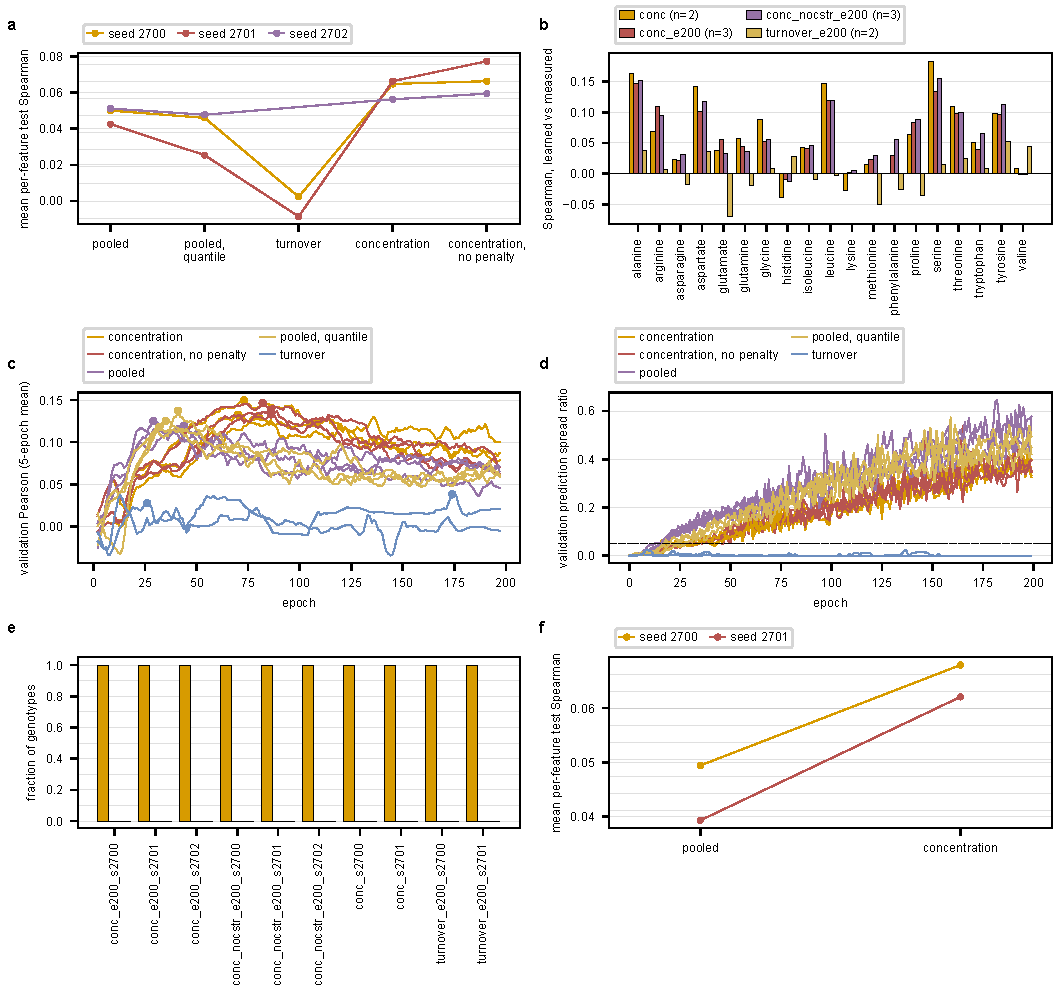
\includegraphics[width=\textwidth]{figures/wave7_aa_concentration.pdf}
  \caption[Wave 7, the amino-acid concentration readout]{\textbf{Supervising the flux
  layer's own whole-cell concentration, against the pooled control.}
  \textbf{a}, Mean per-feature pinned-test Spearman for each readout, one line per seed, so
  a line's slope is the paired difference the contrast table reports. Concentration is above
  pooled at all three seeds and turnover is below it at both of its.
  \textbf{b}, The same statistic per amino acid, learned whole-cell concentration against
  Mulleder's measurement, by arm. The supervised arms run $-0.09$ (histidine) to $+0.17$
  (alanine); the unsupervised turnover arm averages $-0.0031$ over its two seeds, which is
  what says the agreement is supervision rather than physics.
  \textbf{c}, Validation Pearson as a centered five-epoch mean, one line per cell colored by
  its arm, with the selected epoch marked. Selection is on this curve and never on a
  maximum over epochs.
  \textbf{d}, Validation prediction spread ratio per cell, same arm colors, against the
  0.05 collapse line. Every concentration and pooled cell rises away from it; the two
  turnover cells sit on it, which is the collapse panel a shows as a score near zero.
  \textbf{e}, Three component feasibility criteria per flux cell. Mass balance within
  1 percent holds for every genotype in all ten cells, and the flux box and the
  no-uphill-reaction criterion hold for none, drawn as a flat mark at zero beside each unit
  bar. That is the projection parameterization rather than the box one.
  \textbf{f}, The same contrast at the 80-epoch budget, where two seeds have run:
  $+0.0207$, s.d. 0.0030. Generated by
  \texttt{experiments/027-betaxanthin-metabolic/scripts/analyze\_wave7\_aa.py}.}
  \label{fig:wave7-aa}
\end{figure}

\textbf{The learned concentrations are calibrated in level and weak in rank, and the two are
different claims.} Over four orders of magnitude the learned whole-cell medians match the
measured medians to \textbf{0.036 to 0.037 decades}, the mean over the 19 columns across the
three concentration seeds. Per column the held-out Spearman is only $-0.09$ to $+0.17$. A
median that lands and a rank that does not is what a supervised level with little
genotype-to-genotype resolution looks like, and the unsupervised arm's $-0.0031$ says the
level comes from the supervision rather than from the physics.

\textbf{Four caveats, each of which can move the number.} The shipped concentration window
was $[10^{-7}, 10^{-2}]$~M and \textbf{10.63 percent of Mulleder's 88{,}882 measurements sit
above that ceiling}, 9 of the 19 amino acids exceeding it at some strain, so the window was
widened to 1~M before this round; a target on the saturating tail cannot be fit. Five of the
six fractional volumes are assumed rather than sourced, only the nucleus at 0.10 carrying a
citation, so the weights decide which compartment dominates the average and therefore the
physical reading of the prediction. $n = 3$ is three seeds, so the standard deviations here
carry two degrees of freedom and are read for magnitude rather than for a $p$ value. And
this is one endpoint: nothing here says the module helps on betaxanthin.

\subsection{The three readouts, and the control that says the module is off\secstatus{todo}}
\label{sec:aa-readouts}

The amino-acid result above stands or falls on which quantity the 19 predictions are read
from. Three readouts exist, and Figures~\ref{fig:readout-ctx}, \ref{fig:readout-conc} and
\ref{fig:readout-turnover} draw them with the same boxes so the difference is the wiring
and nothing else. \textbf{The flux-coupled concentration readout and its control with no
flux layer at all are the same path from the genotype to the prediction}: both read a
log-concentration vector that is a sigmoid of the pooled context, mix it over compartments,
and score the mixture. The flux enters the second only through the second-law and
dissipation penalties, which reach the concentration vector as a gradient and never reach
the prediction. The turnover readout is the one that reads the flux, and it is the one that
collapses.

\tcfigh[0.98]{figures/aa_readout_context_concentration.pdf}{\textbf{The context-only
  concentration readout (\texttt{context\_concentration}), the control with no flux
  layer.} Orange is the pooled backbone's context vector; purple the sigmoid window that
  turns it into a log concentration for 2{,}806 compartment species and the volume-weighted
  whole-cell mixture over the compartments an amino acid occupies; red the 19 predictions
  and the CRPS loss against Mulleder 2016. No stoichiometry, no kinetic table and no flux
  vector sits on this path.}{fig:readout-ctx}

\tcfigh[0.98]{figures/aa_readout_flux_concentration.pdf}{\textbf{The flux-coupled
  concentration readout (\texttt{flux\_concentration}), the wave-7 arm.} The top row is
  Figure~\ref{fig:readout-ctx} unchanged. Underneath, the same context draws a latent that
  the flux layer (yellow) turns into a flux vector through the box, the $k_{cat}$ capacity
  bound and the mass-balance projection, and the same log concentration sets the reaction
  energies $\Delta_r G' = \Delta_r G^\circ + RT\,S^{\top}\log c$ that price the second-law
  and dissipation terms against that flux at constraint scale 0.1. The dotted edge is the
  only link back: a gradient into the concentration vector. There is no path from the flux
  to the prediction.}{fig:readout-conc}

\tcfigh[0.98]{figures/aa_readout_flux_metabolite.pdf}{\textbf{The turnover readout
  (\texttt{flux\_metabolite}).} The flux is the prediction: context, latent, flux vector,
  then the turnover $\omega_i = \tfrac{1}{2}\sum_j |S_{ij} v_j|$ on the 19 amino-acid rows
  of the stoichiometric matrix, read out directly. It is the only readout that uses the
  module, and it ends as a constant predictor (validation prediction spread 0.000 of the
  target's; jobs 1766 and 1772).}{fig:readout-turnover}

\textbf{Measured on 2026-09-14, the control matches the arm.} The context-only readout on
the pooled backbone reads a mean per-feature pinned-test Spearman of 0.0545, 0.0601 and
0.0670 at seeds 2700 to 2702 (jobs 1899, 1930 and 1931), against the flux-coupled readout's
0.0648, 0.0663 and 0.0562 at the same seeds. Paired by seed the flux-coupled readout is
$+0.0103$, $+0.0062$ and $-0.0108$ above the control, mean $+0.0019$, standard deviation
0.0113, inside the pre-registered kill rule of 0.010. Against the pooled control the
context-only readout is $+0.0127$, which is where the $+0.0145$ of
Section~\ref{sec:wave7-aa} came from: the sigmoid-window parameterization on the pooled
context, not the metabolic module. The flux layer is off for this readout, and the claim
that supervising the layer's own concentration beats the control is withdrawn as a
statement about the layer. The cost of the readout that does use the flux stays: turnover
minus pooled is $-0.0494$ (n = 2), and the wave-6 box flux head is $-0.039$ against pooled
(n = 3). At three seeds the minimum detectable paired effect on this endpoint is about
0.03, so this is a null at every size the design can see rather than a measured zero.

\textbf{How reliable the target is, from the paper's own repeats.} The screen is one culture
per strain, but the raw sheet of Table S3 holds 194 ORFs measured in two batches and 237
injections of a pooled quality-control sample. After per-batch median scaling and a log10,
the two measurements of the same strain correlate at a mean Pearson of 0.43 and a mean
Spearman of 0.20 over the 19 amino acids (glutamine 0.67, glutamate 0.67, proline 0.64 at
the top; glycine 0.12, methionine 0.19, tyrosine 0.20 at the bottom), and the implied
reliability of a single measurement averages 0.42, a Pearson ceiling of about 0.62 for a
perfect predictor of the true value. The quality-control sample disagrees with itself by
only 0.03 to 0.05 log10 units (0.12 for histidine, arginine and tyrosine), while two
cultures of the same strain disagree by 0.16 to 0.27, so the noise is culture-to-culture
rather than instrumental, and it is comparable to the spread across all strains (0.21 to
0.43). Every model in Table~\ref{tab:wave7-aa} and the linear ladder sits at a
mean Spearman of 0.02 to 0.08 against a retest Spearman of 0.20, so the models are far
below what the measurement supports; the target is weak because most deletions move the
pools by less than one culture's worth of noise, not because the assay is. Repeated
strains are the authors' choice rather than a random sample and the scaling omits the
paper's dilution correction, so these are lower bounds on the released table's reliability.
Source: \texttt{mulleder\_retest\_reliability.py}, \texttt{results/mulleder\_retest\_reliability.json}.

%% SOURCE: notes/experiments.027-betaxanthin-metabolic.mermaid.aa-readouts.md (mermaid),
%% rendered by notes/assets/publish/scripts/mermaid_pdf.sh; the numbers are read from
%% experiments/027-betaxanthin-metabolic/results/wave8_aa_ctxconc_e200_s270{0,1,2}.json
%% and wave7_aa_conc_e200_s270{0,1,2}.json (W&B view nw=yxntcreb2vq).

\subsection{What each target can support\secstatus{todo}}

A model cannot correlate with a measurement better than the measurement correlates with
itself. The square root of a target's reliability is therefore the highest Pearson
correlation any predictor of the true level can reach against the stored value, and it is
the number a flat result has to be read against. Six metabolite datasets enter the build and
each releases a different kind of repeat, so each is estimated from its own source rather
than from a shared assumption (Table~\ref{tab:target-reliability}). Three are decoded by a
trained head. The other three are present as genotype context, and their ceilings say which
of them would repay a head of its own.

% notes-tex/027-metabolic-flux-module/tables/target_reliability.tex
%% SOURCE: generated by experiments/027-betaxanthin-metabolic/scripts/target_reliability_table.py
%% from experiments/027-betaxanthin-metabolic/results/target_reliability.json, which that
%% script computes from each dataset's raw release and the two retest result files
%% mulleder_retest_reliability.json and isobutanol_retest_reliability.json.
% Do not edit by hand.
\begin{table}[htbp]
  \centering
  \caption{Reproducibility ceiling of every metabolically relevant target in the 027
  build, each from its own source's repeats. Reliability is the fraction of the variance
  in the stored value that is not measurement noise, and its square root is the highest
  Pearson correlation any predictor of the true level can reach against that stored
  value. The estimator differs by what each release ships: a variance split where it
  gives a mean, a standard deviation and a count; a one-way intraclass correlation where
  it gives repeated raw measurements; a retest correlation where it gives exactly two;
  and a back-solve from the released dispersion where it gives no replicate at all.
  Features is the number of measured quantities the reliability is a median over. The
  lower block enters the build as genotype context, with no head decoding it.}
  \label{tab:target-reliability}
  \footnotesize
  \begin{tabular}{@{}llrrrr@{}}
    \toprule
    Target & Estimator & Repeats & Features & Reliability & Ceiling \\
    \midrule
    \multicolumn{6}{@{}l@{}}{\emph{Read by a trained head}} \\
    Betaxanthin & variance components & 4696 & 1 & 0.84 & 0.92 \\
    Amino acids & retest correlation & 194 & 19 & 0.42 & 0.62 \\
    Isobutanol biosensor & retest correlation & 190 & 1 & 0.11 & 0.33 \\
    \midrule
    \multicolumn{6}{@{}l@{}}{\emph{Present as genotype context only}} \\
    Carotenoid & one-way ICC & 129 & 1 & 0.11 & 0.33 \\
    Metabolome (Zelezniak) & one-way ICC, median over metabolites & 18 & 43 & 0.62 & 0.79 \\
    Lipids (da Silveira) & dispersion back-solve from the released SSMD & 130 & 138 & 0.82 & 0.91 \\
    \bottomrule
  \end{tabular}
\end{table}


\textbf{Betaxanthin is the best measured of the three trained targets, not the worst.} The
CRI-SPA release gives a per-gene mean, standard deviation and colony count over screens 1,
2, 4 and 6, with a median of 15 colonies per gene across the 4{,}696 genes that clear the
paper's own three-colony rule. Splitting the variance into a within-gene and a between-gene
part puts the reliability of the stored gene mean at \textbf{0.84, a Pearson ceiling of
0.92}; one colony on its own carries 0.29, a ceiling of 0.54. Averaging is what buys the
difference. Cachera's own trial-to-trial correlation gives an independent check that lands
in the same place: a reported 0.765 between two trials implies 0.93 for a score combining
four screens by the Spearman-Brown relation, a ceiling of 0.96. The consequence is that the
flat betaxanthin results are not a label-noise story: the nearest-neighbor baseline reads
$+0.145$ pinned Spearman and the module's arms read near zero against a label that supports
far more, so the gap is in the predictor. This estimate assumes colonies of one gene are
independent draws around that gene's level, and a shared plate or position effect would
inflate it.

\textbf{The amino acids sit in the middle}, at a reliability of 0.42 and a Pearson ceiling
of 0.62 with a retest Spearman of 0.20, detailed above.

\textbf{Isobutanol is the weakest genome-wide, and the figure quoted for it earlier was the
wrong one.} The first screen and the validated re-screen agree at Pearson 0.92 over their
225 shared strains, which is the number the research plan used, but the re-screen measured
only strong hits, and selecting the extremes of both tails inflates that correlation: within
the up block alone it falls to 0.41, and within the down block to 0.68. The unselected
estimate comes from 190 genes that appear on two or more rows of the genome-wide screen,
where the two rows correlate at Pearson 0.11 and Spearman 0.31, giving a reliability of 0.11
and a ceiling of 0.33. The pairs are heavy tailed, and dropping the four that disagree by
more than a decade raises the Pearson to 0.29 and a median-based reliability to 0.50, a
ceiling of 0.71. Two things are reproducible even so: direction, with 99.6 percent of
re-screened hits keeping their side of a fold change of 1, and the triplicate re-screen
itself, whose median spread is 0.037 decades against a genome-wide spread of 0.216. The
screen's own disagreement is therefore much larger than culture-to-culture variation in the
re-screen, which is consistent with plate or position effects in a one-shot screen, though
the release carries nothing that separates those from strain-level error.

\textbf{The three context datasets split into two that could carry a head and one that
cannot.} The Zelezniak metabolome reaches a median intraclass correlation of 0.62 over 43
metabolites, a ceiling of 0.79, measured on the two protocols that re-grew independent
cultures; the protocol covering all 96 genotypes carries no replicate at all, and the two
that do re-grew only strains that varied in the first, so the estimate comes from a
deliberately variable subset. The da Silveira lipids release no replicate either, and
recovering the within-mutant spread from the released strictly standardized mean difference
puts the median per-lipid reliability at 0.82 over 138 lipids, a ceiling of 0.91. That is
the weakest estimate in the table, because it inherits whatever definition the dispersion
column was computed under rather than measuring a repeat.

\textbf{The carotenoid screen is the one context target whose label cannot support a head.}
Ozaydin 2013 scores colony color on a 6-level visual scale, and 129 strains appear in more
than one batch. Their intraclass correlation is \textbf{0.11, a ceiling of 0.33}, the
weakest label of the six and the same magnitude as the isobutanol screen. The published
second round of transformations cannot extend that estimate, because it re-screened only
strains that had already scored 2.5 or higher. A coarse ordinal score read by eye is what
this bound is measuring, so the limit is the assay rather than the biology.

\textbf{Essentiality is bounded differently, and its bound is high.} The fourth endpoint the
module now trains on is gene essentiality, whose label comes from the yeast split released
with Merzbacher 2025, the same file the published comparator numbers were computed on. A
binary label has no correlation ceiling, so the analogous bound is how far two independently
curated sources agree: a predictor that reproduced one perfectly would score that agreement
against the other. Over the split's 1{,}121 genes, the Saccharomyces Genome Database
essential-gene list disagrees with the split on 13, eleven that the database calls essential
and the split does not, and two the other way, for an agreement of \textbf{98.8 percent
against a majority rate of 86.0 percent}. Nearly 13 points of headroom separate a constant
predictor from the label's own limit, which is far more room than any of the three
metabolite targets offers. The database list carries no negative class, so absence from it
counts as nonessential only for genes the split names.

Ordering the three trained metabolite targets by headroom puts betaxanthin first, the amino
acids second and isobutanol last, which reverses the ranking the research plan used when it
called isobutanol the best-conditioned target. Across all six, betaxanthin and the lipids
are the labels that can support a strong correlation, and the carotenoid and isobutanol
screens are the two that cannot.

The table is built by \texttt{target\_reliability\_table.py} into the result file
\texttt{target\_reliability.json}. The isobutanol repeats are measured by
\texttt{isobutanol\_retest\_reliability.py}, and the amino-acid repeats by the script named
in the paragraph above. The essentiality comparison is
\texttt{essentiality\_label\_agreement.py}. Every result file sits in the experiment's
\texttt{results} directory.

\subsection{Betaxanthin parity, and the criterion that has never been met\secstatus{todo}}

On the endpoint the module was built for, the same wave is flat. \textbf{Betaxanthin parity
on the one shipped kinetic table is $-0.055$ pinned-test Spearman, standard deviation 0.090
over three seeds}, scored at the epoch the centered five-epoch moving average of validation
Pearson selects. A mean of that size against a standard deviation of that size is a null
result rather than a cost, and it is what the amino-acid round is measured beside.

\textbf{The Genesis criterion has never been met under an honest rule.} Across all 18 cells
audited, the fraction of genotypes meeting it is \textbf{0.0} under the median rule, under
the max rule and under the flux-active rule alike. It is met by 4 of the 12 cells that carry
the number only under the variant scored against the model's own thermodynamics rather than
the standard state, which is the rule that grades the model against itself.
%% SOURCE: experiments/027-betaxanthin-metabolic/results/wave7_parity_summary.json, keys
%% `wave7` (n_pairs 3, mean_difference, sd_difference) and `feasibility`
%% (genesis_median_rule, genesis_max_rule, genesis_active_rule,
%% genesis_median_rule_model_thermo); written by analyze_wave7_parity.py.
